\documentclass[12px]{article}
\usepackage[cjk]{kotex}
\usepackage[top=2cm, bottom=4.5cm, left=2.5cm, right=2.5cm]{geometry}
\usepackage{amsmath, amssymb}
\usepackage{enumerate}
\usepackage{graphicx}
% \usepackage{tikz}
% \addtolength{\oddsidemargin}{-.875in}
% \addtolength{\evensidemargin}{-.875in}
% \addtolength{\textwidth}{1.75in}
% \addtolength{\topmargin}{-.875in}
% \addtolength{\textheight}{1.75in}

\title{응용통계학 5장 연습문제 풀이}
\author{20181653 이강희}
\date{}

\begin{document}
\maketitle

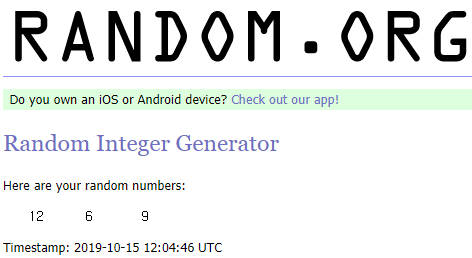
\includegraphics[scale=0.7]{random}

\section*{6번}
20개를 비복원 추출하므로 $X$는 초기하분포를 따른다.
\begin{enumerate}[(1)]
    \item
    \begin{minipage}[t]{\linewidth}
    \vspace{-\baselineskip}
    \begin{flalign*}
        f(x) &= \frac{{\binom{10}{x} \binom{490}{20-x}}}{\binom{500}{20}}, x = 0,1,2,\dots,10&
    \end{flalign*}
    \end{minipage}
    \item
    \begin{minipage}[t]{\linewidth}
    \vspace{-\baselineskip}
    \begin{flalign*}
        E(X) &= \frac{nr}{N} = \frac{20\times 10}{500} = \frac{2}{5}&\\
        V(X) &= np(1-p)(\frac{N-n}{N-1})\\
        &= 20 \times \frac{1}{50} \times \frac{49}{50} \times \frac{480}{499}\\
        &\approx 0.377
    \end{flalign*}
    \end{minipage}
    \item
    \begin{minipage}[t]{\linewidth}
    \vspace{-\baselineskip}
    \begin{flalign*}
        f(2) &= \frac{\binom{10}{2} \binom{490}{18}}{\binom{500}{20}} \approx 0.0509&
    \end{flalign*}
    \end{minipage}
    \item
    \begin{minipage}[t]{\linewidth}
    \vspace{-\baselineskip}
    \begin{flalign*}
        P(X\leq 2) &= \sum_{x=0}^{2} \frac{\binom{10}{x} \binom{490}{20-x}}{\binom{500}{20}}&\\
        &\approx 0.6623 + 0.2812 + 0.0509\\
        &= 0.9944
    \end{flalign*}
    \end{minipage}
\end{enumerate}

\section*{9번}
\begin{enumerate}[(1)]
    \setlength\abovedisplayskip{0pt}
    \item
    불량이 나올때까지 검사개수는 기하분포를 따른다.
    \begin{flalign*}
        E(X) &= \frac{1}{p} = \frac{1}{0.01} = 100&\\
        V(X) &= \frac{q}{p^2} = \frac{0.99}{0.01^2} = 9900\\
        \sigma_x &= \sqrt{9900} \approx 99.4987
    \end{flalign*}
    \item
    50개의 제품을 검사할 때까지 불량이 나오지 않을 확률은
    \begin{flalign*}
        P(X > 50) &= 0.99^{50} \approx 0.605&
    \end{flalign*}
    \item
    기하분포는 비기억특성을 갖기때문에,
    \begin{flalign*}
        P(X > 50+50 \mid X > 50) &= P(X > 50)&\\
        &\approx 0.605
    \end{flalign*}
\end{enumerate}

\section*{12번}
다항분포이다.
\begin{enumerate}[(1)]
    \item
    1루타 2개, 2루타 3개, 홈런 4개가 정해지면 나머지 1개는 3루타라는 것을 알 수 있다.
    \begin{flalign*}
        \frac{10!}{2!3!4!1!}0.2^2 0.3^3 0.4^4 0.1 &= 0.03483648&\\
    \end{flalign*}
    \item
    2루타 3개, 홈런 4개와 나머지 3개로 나눌 수 있다.
    \begin{flalign*}
        \frac{10!}{3!4!3!}0.3^3 0.4^4 0.3^3 &= 0.07838208&\\
    \end{flalign*}
    \item
    홈런 4개와 나머지 6개로 나눌 수 있다.
    \begin{flalign*}
        \frac{10!}{4!6!}0.4^4 0.6^6 &= 0.250822656&\\
    \end{flalign*}
    \item
    3번의 확률이 가장 높고, 3번, 2번, 1번 순으로 확률이 높다.\\
    속성의 개수 $k$ (확률변수의 개수)가 적어질수록 확률이 높아진다.
    \item
    $X\sim NB(0.4, 10)$ 인 확률변수 $X$에서,
    \begin{flalign*}
        \sum_{x=4}^{10} f(x) &= \sum_{x=4}^{10} \binom{x-1}{3} 0.4^4 0.6^{x-4}&\\
        &= \binom{3}{3} 0.4^4 0.6^0 + \binom{4}{3} 0.4^4 0.6^1 + \dots + \binom{9}{3} 0.4^4 0.6^6\\
        &= 0.6177193984
    \end{flalign*}
\end{enumerate}

\end{document}